\section{Profunctors and the Gro\-then\-dieck construction}\label{sec_2_profu}
\label{sec:org7dd09e1}
There are two possible ways to define a \emph{relation} $R$ between two sets $A,B$:
\begin{enumtag}{r}
  \item \label{r_1} a relation $R$ is a subset of the cartesian product $A\times B$;
  \item \label{r_2} a relation $R$ is a function $A\times B \to \{0,1\}$.
\end{enumtag}
This notion of `relation between $A$ and $B$' is inherently symmetric, in the sense that such $R$ can be regarded both as a kind of `botched' map $A \rightsquigarrow B$ or $B\rightsquigarrow A$: a relation between $A$ and $B$ is equally a function $B\to PA$ or $A\to PB$.

Because of this, every relation $R$ between sets $A,B$ gives rise to a \emph{Galois connection}
\[{}^R(\firstblank) :PA^\op \leftrightarrows PB : (\firstblank)^R \label{adjunzia} \]
between the power-sets $PA=2^A$ and $PB = 2^B$: the set $U\subset A$ goes to the set ${}^RU$ of all $b$ such that $(a,b)\in R$ for all $a\in U$; in an exactly symmetric way, a set $V\subseteq B$ goes to the set
\[V^R = \{a\in A\mid (a,b) \in R,\, \forall b\in V\}.\]
Unwinding the definition, it is easy to verify that $V\subseteq{}^RU$ if and only if $U\subseteq V^R$, if and only if $U\times V\subseteq R$, so the adjunction rules of \cite[3.1.6m]{Bor1} are satisfied.
%\todo[inline]{La varianza di sta roba va controllata}

Now, using a process known as `categorification' \cite{baez1998categorification}, we can replace a \emph{two-valued} relation $R : A\times B \to \{0,1\}$ with a \emph{set-valued} functor $\clA^\op\times\clB \to \Set$ between two (small) categories $\clA,\clB$.\footnote{The reason why the category $\clA$ is twisted with an `$^\op$' functor is that we want to bestow the hom functor $\hom_{\clA} : \clA^\op\times\clA \to \Set$ with the r\^ole of identity `profunctor'; in the categorification perspective, hom plays the r\^ole of the diagonal relation $R=\Delta : A\to A\times A$. The category of sets (i.e., of discrete categories) has no nontrivial involution on objects, so in the case of sets the opping operation is hidden.} In this perspective, the truth value for the proposition $aRb$=`$(a,b) \in R$' is considered too poor an information about $R$ (it is also usually wise to approach mathematics rejecting two-valued logic); because of this, instead of the mere truth value of the proposition $aRb$ we consider the \emph{type} of all \emph{proofs} that $aRb$. This point of view will be re-introduced along \autoref{sec_5_tension}.

More precisely, we can give the following definition.
\begin{definition}[Profunctor]\label{def_profu}
  Let $\clA,\clB$ be two small categories; a \emph{profunctor} $\fkR : \clA \pto \clB$ is, by definition, a functor $\clA^\op\times\clB \to \Set$; we define the \emph{bicategory of profunctors} $\Prof$ having
  \begin{enumtag}{p}
    \item objects the small categories $\clA,\clB,\clC,\dots$;
    \item 1-cells the profunctors $\fkR : \clA \pto \clB$, and composition law between $\clA \overset{\fkR}{\pto} \clB \overset{\fkP}{\pto} \clC$ given by the assignment\footnote{See \cite[6.2.10]{Bor2} for the definition: representing a profunctor as a matrix of sets, this universal construction is the matrix product whose $(A,C)$-entry is the generalised sum $\sum_B \fkR(A,B)\times\fkP(B,C)$ modded out for a certain equivalence relation.}
    \[ \fkP\diamond \fkR : (A,C)\mapsto \int^B \fkR(A,B)\times\fkP(B,C) \]
    \item the identity 1-cell is the hom functor $\hom_\clA : \clA^\op\times\clA \to \Set$;
    \item 2-cells $\fkR\To\fkR'$ the natural transformations $\alpha : \xymatrix{**[l] \clA^\op\times\clB \rtwocell^{\fkR}_{\fkR'}{\alpha}& **[r] \Set}$.
  \end{enumtag}
\end{definition}
This formalises the above intuition that $\fkR(A,B)$ is the \emph{type} whose terms are all proofs that $(A,B)\in\clA^\op\times\clB$ are in a  `generalised relation' $\fkR$. This intuition agrees with the fact that a profunctor between discrete categories is precisely a relation between the sets that those two categories are.

Starting from here, one can build a rich and expressive theory; for our purposes, we are contempt with a careful analysis of the analogue of \ref{r_2} and \eqref{adjunzia} above: the latter is the scope of \autoref{sec:org1a423df}, we now concentrate on describing a ubiquitous technical tool in category theory, called \emph{Gro\-then\-dieck construction}, suited to categorify the equivalence between \ref{r_1} and \ref{r_2}.

Every function is a particular relation: this means that the category of sets and functions embed into the category of relations and that a relation is just a function satisfying a suitable rigidity request; something similar happens to profunctors, and we will freely employ the notation that the following definition sets up throughout the paper (cf. for example \autoref{uan}, \autoref{ciu}, \autoref{funcell_herme}).
\begin{definition}[The upper and lower image of a functor]\label{upper_n_lower}
  Let $F : \clA \to \clB$ be a functor; we define 
  \begin{enumtag}{im}
    \item the \emph{upper image} $F^*$ of $F$ is $\Prof$ to be the functor 
    \[ \clB(F,1) : \clA^\op\times\clB \to\Set : (A,B)\mapsto \clB(FA,B) \]
    \item the \emph{lower image} $F_*$ of $F$ is $\Prof$ to be the functor 
    \[ \clB(1,F) : \clB^\op\times\clA \to\Set : (B,A)\mapsto \clB(B,FA) \]
  \end{enumtag}
  The correspondence $F\mapsto F^*$ is a functor, covariant on 1-cells and contravariant on 2-cells; the correspondence $F\mapsto F_*$ is a functor, contravariant on 1-cells, and covariant on 2-cells.
\end{definition}
\subsection{Gro\-then\-dieck construction}
Each profunctor $\fkR : \clA \pto \clB$ can be realised as a suitable `fibration' $p_\fkR : \clE \to \clA^\op\times\clB$, that in turn uniquely determines $\fkR$.
We now recall a few basic definitions.
\begin{definition}\label{eltsf}
  Let $\clC$ be an ordinary category, and let $W : \clC\to \Set$ be a functor; the \emph{category of elements} $\elts{\clC}{W}$ of $W$ is the category which results from the pullback
  \[
    \vcenter{\xymatrix{
      \elts{\clC}{W}\ar[r]\ar[d] \pb & \Set_* \ar[d]^U \\
      \clC \ar[r]_W & \Set
    }}
  \]
  where $U : \Set_*\to\Set$ is the forgetful functor which sends a pointed set to its underlying set.

  More explicitly, $\elts{\clC}{W}$ has objects the pairs $(C\in\clC, u\in WC)$, and morphisms $(C,u)\to (C',v)$ those $f\in \clC(C,C')$ such that $W(f)(u)=v$.
\end{definition}
\begin{definition}[Discrete fibration]
  \label{def:dfib}
  A \emph{discrete fibration} of categories is a functor $G : \clE \to \clC$ with the property that for every object $E\in\clE$ and every arrow $p : C\to GE$ in $\clC$ there is a unique $q : E'\to E$ `over $p$', i.e. such that $Gq=p$.
\end{definition}
Taking as morphisms between discrete fibrations the morphisms in $\Qat/\clC$, we can define the category $\DFib(\clC)$ of discrete fibrations \emph{over} $\clC$.
\begin{proposition}\label{fibelem}
  The category of elements $\elts{\clC}{W}$ of a functor $W : \clC\to \Set$ comes equipped with a canonical \emph{discrete fibration} to the domain of $W$, which we denote $\Sigma : \elts{\clC}{W}\to \clC$, defined forgetting the distinguished element $u\in WC$.
\end{proposition}
With this terminology at hand, we can consider the category of elements of a functor $F : \clC\to \Set$; this sets up a functor from $\Qat(\clC,\Set)$ to the category of discrete fibrations over $\clC$: the Gro\-then\-dieck construction asserts that this is assignment sets up an equivalence of categories.%, as defined in \ref{def:equcat}.
\begin{theorem}\label{thm:equconfib}
  There is an equivalence of categories
  \[
    \Qat(\clC^\op,\Set) \to \DFib(\clC)
  \]
  defined by the correspondence sending $F\in\Qat(\clC,\Set)$ to its \emph{fibration of elements}  $\Sigma_F : \elts{\clC}{F} \to \clC$.
\end{theorem}
The inverse correspondence sends a discrete fibration $\Phi : \clE \to \clC$ to the functor whose action on objects and morphisms is depicted in the following image: an object $C\in\clC$ goes to the fiber $\Phi^{-1}C$ in $\clE$, that since $\Phi$ is a discrete fibration is a discrete subcategory of $\clE$, hence a set; a morphism $u : C\to C'$ defines a function $\Phi^{-1}C' \to \Phi^{-1}C$: the object $X'\in\Phi^{-1}C'$ goes to the (unique) object $X$ in the fiber over $C$, that is the domain of the arrow $v$ such that $\Phi v=u$.
\begin{center}
  % 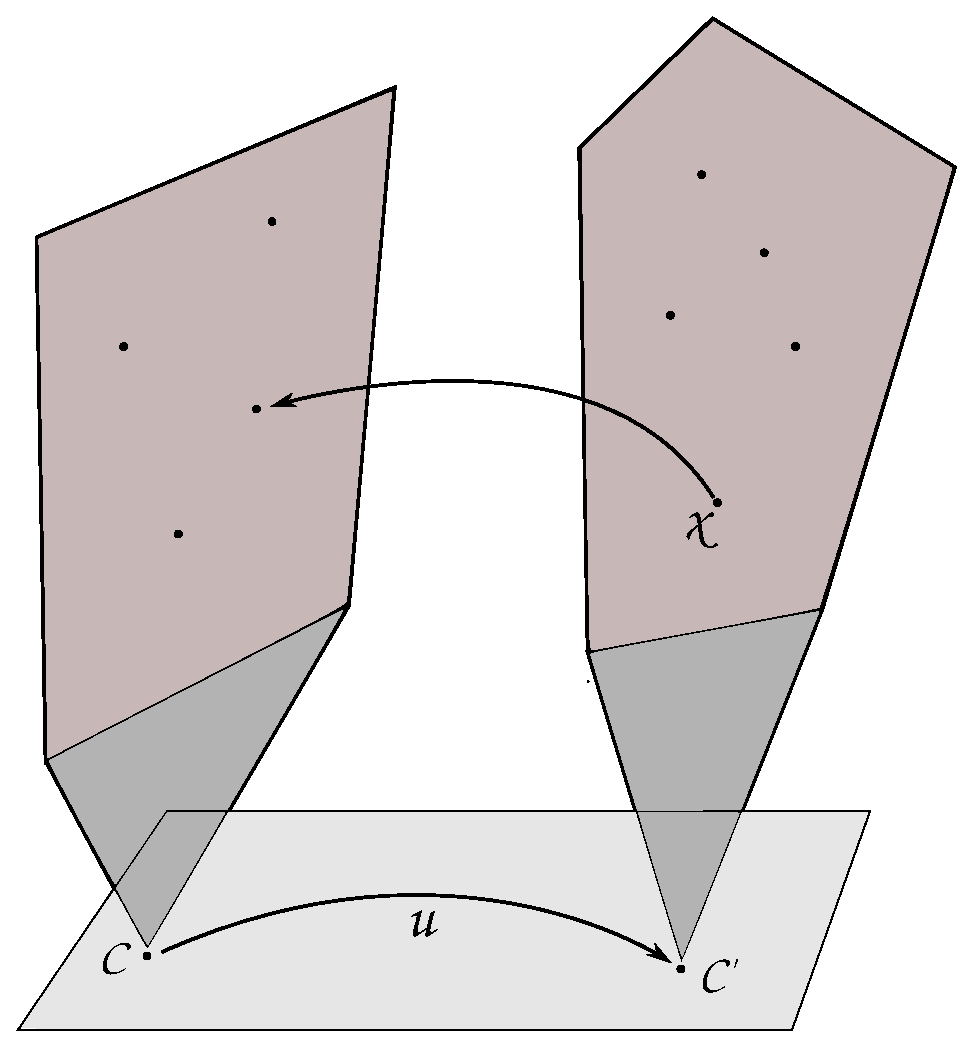
\includegraphics[width=.325\textwidth]{disegno.eps}
  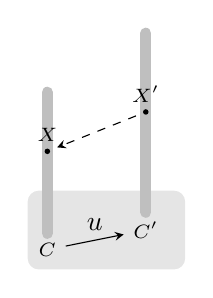
\begin{tikzpicture}[>=stealth]
    \fill[gray!20,rounded corners] (0,0) rectangle (2,1);
    \node[font=\scriptsize] (C) at  (.25,.25) {$C$};
    \node[font=\scriptsize] (C') at (1.5,.5)  {$C'$};
    \draw[->] (C) -- (C') node[above, pos=.5] {$u$};
    %
    \draw[line width=4pt, gray!50, cap=round] (C) -- +(0,2);
    \draw[line width=4pt, gray!50, cap=round] (C') -- +(0,2.5);
    %
    \fill (1.5,2) circle (1pt) node (X') {};
    \fill (.25,1.5) circle (1pt) node (X) {};
    \draw[dashed,->] (X') -- (X);
    \node[above, font=\scriptsize] at (X') {$X'$};
    \node[above, font=\scriptsize] at (X) {$X$};
  \end{tikzpicture}
\end{center}
There is of course a similar correspondence for \emph{covariant} functors; the situation is conveniently depicted by the table
\begin{center}
  \begin{tabular}{ccc}
    \textbf{name}       & \textbf{variance}   & \textbf{condition} \\ \toprule
    fibration           & $\clC\to\Set$       &
    $
      \vcenter{\tiny \xymatrix@R=5mm{
    X \ar[r] \ar@{.}[d] & X'\ar@{.}[d]                             \\ \midrule
    pX \ar[r]_f         & C'
      }}
    $
    \\ \midrule
    opfibration         & $\clC^\op \to \Set$ &
    $
      \vcenter{\tiny \xymatrix@R=5mm{
    X \ar[r] \ar@{.}[d] & X'\ar@{.}[d]                             \\ \midrule
    C \ar[r]_f          & pX'
      }}
    $
    \\ \bottomrule
  \end{tabular}
\end{center}
% \f{La notazione va uniformata a questa scelta}
\begin{corollary}\label{da_collage}
  Given a profunctor $\fkR : \clA \pto \clB$, regarded as a functor $R : \clA^\op\times \clB \to \Set$, we can consider the category of elements $\elts{\clA^\op\times\clB}{R}$; this is often called the \emph{collage} or the \emph{graph} of $R$. In this case, we denote the category $\elts{\clA^\op\times\clB}{R}$ as $\clA\uplus_R\clB$, to stress the intuition that $R$ prescribes a way to glue together two categories $\clA,\clB$ specifying a set of `fake' arrows $R(A,B)$ that consistently interact with the arrows in $\clA,\clB$ (compare this with \autoref{11_ramsey} below).
\end{corollary}
\begin{remark}\label{collage_explaned}
  The above definition deserves to be expanded a little more: from \autoref{eltsf} we get that the category $\clA\uplus_R\clB$ results as the category whose objects are those of the disjoint union $\clA_o\sqcup\clB_o$, and where the hom-set $\clA\uplus_R\clB(X,Y)$ is equal to
  \begin{enumtag}{c}
    \item $\clA(A,A')$ if $(X,Y)=(A,A')$ is a pair of objects in $\clA$;
    \item $\clB(B,B')$ if $(X,Y)=(B,B')$ is a pair of objects in $\clB$;
    \item $R(A,B)$ if $X=A$ is an object of $\clA$, and $Y=B$ is an object of $\clB$;
    \item empty in every other case.
  \end{enumtag}
  From this definition, it is evident that every profunctor $\fkR : \clA \pto \clB$ gives rise via its fibration of elements to a span of categories
  \[ \vcenter{\xymatrix{
        & \clA\uplus_\fkR \clB \ar[dr]\ar[dl]& \\
        \clA^\op  && \clB
      }} \]
\end{remark}
Thus, we have obtained a concrete model for a category that realises the generalised relation between $\clA,\clB$; the structure $\clA\uplus_R\clB$ is `carved' from $\clA,\clB$ separately, starting from (semi-)free relations witnessing the fact that $\fkR$ connects $\clA,\clB$ in a weak way. For example, if $\fkR : \clA^\op\times \clB \to \Set$ is the empty functor, then $\clA\uplus_R\clB$ is just he disjoint union of $\clA,\clB$; and if $\fkR$ is the functor constant at the singleton set, then $\clA\uplus_R\clB$ is the \emph{join} of $\clA,\clB$, i.e. the category $\clA\coprod\clB$ where exactly a single new morphism is added between each and every object of $\clA$ and of $\clB$ (but not in the opposite direction).

As a final remark, we observe that the extremely rich features of the Grothendieck construction can be at least partly explained resorting to a dual construction for $\elts{\clC}{F}$: more in detail,
\begin{proposition}\label{uan}
  The collage construction of \autoref{da_collage} enjoys the following universal property: the category $\clA\uplus_R\clB$ fits into a cospan
  \[ \xymatrix{\clA \ar[r]^-J & \clA\uplus_R\clB & \ar[l]_-K \clB} \]
  where both functors $J,K$ are the obvious embeddings, and there exists a canonical natural transformation $\gamma : K_* \diamond \fkR \To J_*$ which is initial among all these: this means that given any other arrangement of profunctors 
  \[ \vcenter{\xymatrix{
    \clA \ar|-*=0@{|}@/^1pc/[drr]^(.6)\fkP\ar|-*=0@{|}[dr]^{J_*}\ar|-*=0@{|}[dd]_\fkR && \\ 
    & \clA\uplus_R\clB \ltwocell<\omit>{\gamma} \ar|-*=0@{|}@{.>}[r]^-{\fkU}& \clC \\ 
    \clB \ar|-*=0@{|}[ur]_{K_*}\ar|-*=0@{|}@/_1pc/[urr]_(.6)\fkQ & 
  }} \] like in this diagram of solid arrows, there exists a unique profunctor $\fkU : \clA\uplus_R\clB \pto \clC$ such that $\fkU\diamond J_*=\fkP$, $\fkU\diamond K_* = \fkQ$, and $\fkU * \gamma = \alpha$.
\end{proposition}